\documentclass[12pt]{article}
\usepackage{amsmath}
\usepackage{amsfonts}
\usepackage{amssymb}
\usepackage{mathabx}
\usepackage{graphicx}
\usepackage{graphicx}
\usepackage{subfig}
\usepackage{multirow}
\usepackage{array}
\usepackage[margin=4cm]{geometry}
\usepackage{fancybox}
% Default margins are too wide all the way around.  I reset them here
\setlength{\topmargin}{-.5in}
\setlength{\textheight}{9in}
\setlength{\oddsidemargin}{.125in}
\setlength{\textwidth}{6.25in}
\newenvironment{wideverbatim}%
{\vskip\baselineskip\VerbatimEnvironment
\begin{Sbox}\begin{BVerbatim}}
{\end{BVerbatim}%
\end{Sbox}\noindent\centerline{\TheSbox}\vskip\baselineskip}
\begin{document}
\title{Taller 2 se\~nales y sistemas}
\author{Sebasti\'an Valencia Calder\'on\\
Universidad de los Andes}
\renewcommand{\today}{Febrero 26, 2013}
\maketitle
\begin{enumerate}
\item  Calcule la DFT de las siguientes se\~nales $
\boldsymbol{\vec{u}}=[1,0,0,0,0]$, $\boldsymbol{\vec{v}}=[0,1,0,0,0]$,
$\boldsymbol{\vec{w}}=[0,0,1,0,0]$, $\boldsymbol{\vec{x}}=[0,0,0,1,0]$ y
$\boldsymbol{\vec{y}}=[0,0,0,0,1]$.
Grafique la magnitud y la fase de las
transfromadas.

La DFT, se define con la siguiente regla de transformaci\'on, donde $x_n$ es la
n-\'esima posici\'on del vector a transformar o de la entrada, y $X_n$ la
n-\'esima posici\'on del vector transfromado o la salida.

$$\mbox{\bf{DFT}\rm}[z_k]=Z_k=\sum_{n=0}^{N-1}
z_ne^{{\frac{-i2n\pi}{N}}k}$$
A cada vector o se\~nal discreta se le aplicar\'a la regla de transformaci\'on
para obtener la respectiva DFT, a continuaci\'on se muestra el proceso
algor\'itmico de cada transformaci\'on. Para las cinco se\~nales, se tiene que
su longitud $N$ es cinco, por lo tanto la regla de transformaci\'on de un
vector de entrada $z$ estar\'a dada por la igualdad anterior con $N=5$. Ya que
los vectores tienen magnitud uno por tener un \'unico elemento unitario en \'el,
la deducci\'on formal de la transformada, se reduce a evaluar la expresi\'on
$e^{{\frac{-i2n\pi}{N}}k}$ para $n$ igual a la posici\'on de la entrada unitaria del
vector, comenzando el conteo de posici\'on en cero.


$$U_k=e^{{\frac{-i2(0)\pi}{5}}k}=[e^{{\frac{0}{5}}},
e^{{\frac{0}{5}}}, e^{{\frac{0}{5}}}, e^{{\frac{0}{5}}},
e^{{\frac{0}{5}}}]=[1, 1, 1, 1, 1] $$
$$V_k=e^{{\frac{-i2(1)\pi}{5}}k}=[e^{{\frac{-i2\pi}{5}}0},
e^{{\frac{-i2\pi}{5}}1}, e^{{\frac{-i2\pi}{5}}2}, e^{{\frac{-i2\pi}{5}}3},
e^{{\frac{-i2\pi}{5}}4}]=[1, e^{{\frac{-i2\pi}{5}}},
e^{{\frac{-i4\pi}{5}}},e^{{\frac{-i6\pi}{5}}},e^{{\frac{-i8\pi}{5}}}]$$
$$W_k=e^{{\frac{-i2(2)\pi}{5}}k}=[e^{{\frac{-i4\pi}{5}}0},
e^{{\frac{-i4\pi}{5}}1}, e^{{\frac{-i4\pi}{5}}2}, e^{{\frac{-i4\pi}{5}}3},
e^{{\frac{-i4\pi}{5}}4}]=[1, e^{{\frac{-i4\pi}{5}}},
e^{{\frac{-i8\pi}{5}}},e^{{\frac{-i12\pi}{5}}},e^{{\frac{-i16\pi}{5}}}]$$
$$X_k=e^{{\frac{-i2(3)\pi}{5}}k}=[e^{{\frac{-i6\pi}{5}}0},
e^{{\frac{-i6\pi}{5}}1}, e^{{\frac{-i6\pi}{5}}2}, e^{{\frac{-i6\pi}{5}}3},
e^{{\frac{-i6\pi}{5}}4}]=[1, e^{{\frac{-i6\pi}{5}}},
e^{{\frac{-i12\pi}{5}}},e^{{\frac{-i18\pi}{5}}},e^{{\frac{-i24\pi}{5}}}]$$
$$Y_k=e^{{\frac{-i2(4)\pi}{5}}k}=[e^{{\frac{-i8\pi}{5}}0},
e^{{\frac{-i8\pi}{5}}1}, e^{{\frac{-i8\pi}{5}}2}, e^{{\frac{-i8\pi}{5}}3},
e^{{\frac{-i8\pi}{5}}4}]=[1, e^{{\frac{-i8\pi}{5}}},
e^{{\frac{-i16\pi}{5}}},e^{{\frac{-i24\pi}{5}}},e^{{\frac{-i32\pi}{5}}}]$$

Para facilitar el proceso de graficaci\'on, se usar\'a la forma rectangular de
cada elemento. Puesto que es m\'as f\'acil de considerar la magnitud y la fase
dada esta forma. La anterior descripci\'on, resulta muy tediosa si se hace con
una calculadora, por lo tanto, se ahorra tiempo implementando un algoritmo en
MATLAB que para cada vector de entrada de tama\~no N, arroja su DFT; el
algoritmo es el siguiente (El algoritmo, fue dise\~nado por John Proakis, se
encuentra en MATLAB central. No se incluyen comentarios por su sencillez.)

\begin{verbatim}
function [Xk] = dft(xn,N)
n = [0:1:N-1];      
k = [0:1:N-1];                    
WN = exp(-j*2*pi/N);               
nk = n'*k;                           
WNnk = WN .^ nk;                     
Xk = xn * WNnk;                        
\end{verbatim}

La implementaci\'on en MATLAB del anterior algoritmo, para cada se\~nal da los
siguientes resultados, donde a,b,c,d,e son los vectores $\boldsymbol{\vec{u}},
\boldsymbol{\vec{v}}, \boldsymbol{\vec{w}}, \boldsymbol{\vec{x}},
\boldsymbol{\vec{y}}$ respectivamente y N es cinco.
{\tiny
\begin{verbatim}
>> dft(a,N)
ans =

     1     1     1     1     1

>> dft(b,N)
ans =

   1.0000  0.3090 - 0.9511i  -0.8090 - 0.5878i  -0.8090 + 0.5878i   0.3090 + 0.9511i

>> dft(c,N)
ans =

   1.0000  -0.8090 - 0.5878i   0.3090 + 0.9511i   0.3090 - 0.9511i  -0.8090 +
   0.5878i

>> dft(d,N)
ans =

   1.0000 -0.8090 + 0.5878i   0.3090 - 0.9511i   0.3090 + 0.9511i  -0.8090 - 0.5878i

>> dft(e,N)
ans =

   1.0000  0.3090 + 0.9511i  -0.8090 + 0.5878i  -0.8090 - 0.5878i   0.3090 - 0.9511i

>> 
\end{verbatim}
}
Ahora que se conocen las transformadas de las funciones y un m\'etodo
computacional para hacerlo, se grafica tambi\'en con MATLAB la magnitud y la
fase de la transformada. En la siguiente disposici\'on de figuras, es posible
ver que para el tercer vector, la fase de su DFT obedece su naturaleza de funci\'on
multivaluada, es decir que para un valor de $n$ puede tomar varios valores de la
variable dependiente. Asimismo, puede verse que la amplitud de cada DFT es uno
para todos los valores de $n$, lo cual era de esperarse por el factor
multiplicativo de la expresi\'on $e^{{\frac{-i2n\pi}{N}}k}$ para cada
transfromada, el cual es uno.
\\
Para la obtenci\'on de las gr\'aficas, usando la forma rectangular de cada
elemento del vector de salida, se hall\'o con la funcion dise\~nada de MATLAB
\bf{cart2poly(a,b)}\rm para un n\'umero complejo $a+ib$,
\begin{figure}
\centering
\begin{tabular}{cc}
\subfloat[DFT-A]{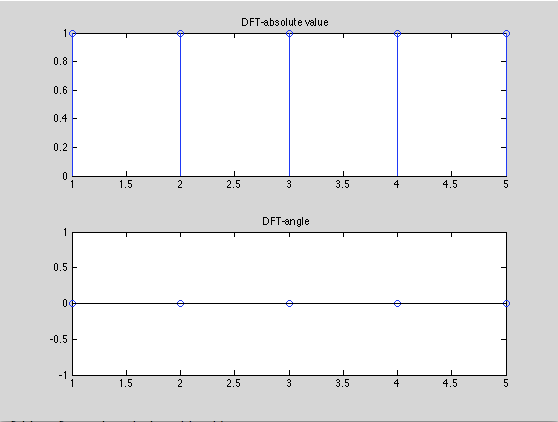
\includegraphics[scale=0.35]{1.png}} & 
\subfloat[DFT-B]{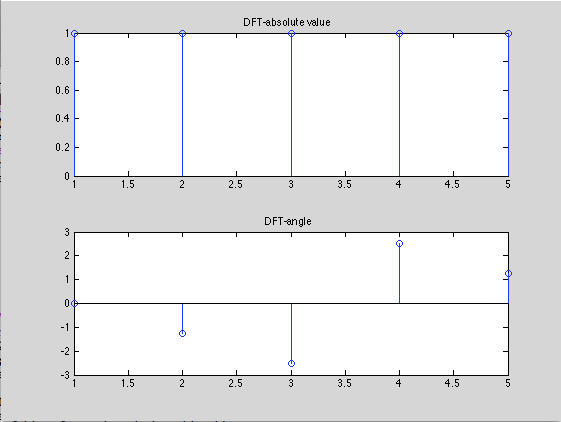
\includegraphics[scale=0.35]{2.png}} \\ 
\subfloat[DFT-C]{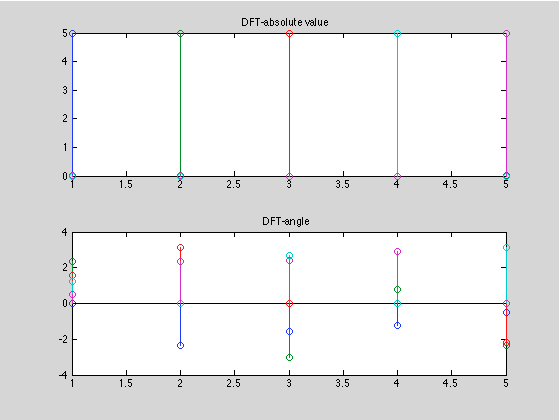
\includegraphics[scale=0.35]{3.png}} &
\subfloat[DFT-D]{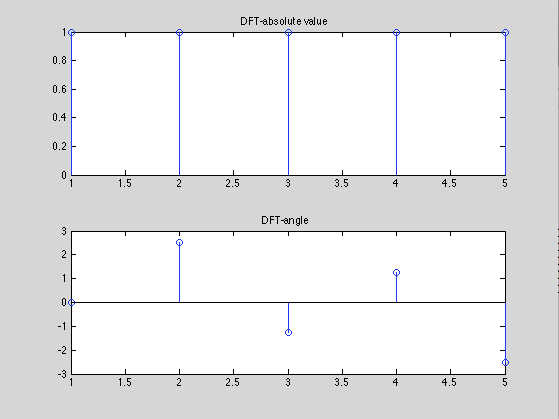
\includegraphics[scale=0.35]{4.png}}\\
\subfloat[DFT-E]{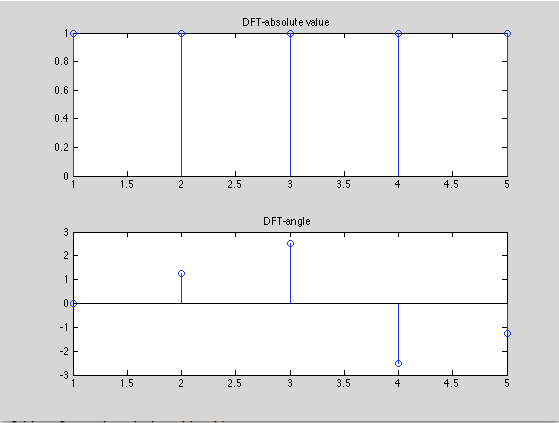
\includegraphics[scale=0.35]{5.png}}\\
\end{tabular}
\caption{Gr\'aficos de amplitud magnitud de la DFT de cada vector}
\end{figure}
\pagebreak
\item Con base en la definici\'on de la DFT, muestre que la transformada de la
se\~nal $y_n=x_{[n+m]} \bmod N$ est\'a dada por $Y_k=e^{{\frac{i2m\pi}{N}}k}X_k$
Explique los resultados del punto anterior a la luz de esta propiedad de
corrimiento de la DFT.

Sea $\boldsymbol{\vec{x}}=[x_0,x_1,\ldots,x_{N-1}]$ una se\~nal de $N$ entradas,
sea $\boldsymbol{\vec{X}}=[X_0,X_1,\ldots,X_{N-1}]$ su DFT. Si se define la
se\~nal $y$ como un corrimiento modular de la se\~nal $x$ de la forma
$\boldsymbol{\vec{y}}=[x_m,x_{m+1},\ldots,x_{m-1}]$, se tiene que la
transformada de este vector modificado ser\'a:
$$\mbox{\bf{DFT}\rm}[y_k]=Y_k=\sum_{n=0}^{N-1}
y_ne^{{\frac{-i2n\pi}{N}}k}=\sum_{n=0}^{N-1}
x_{[n+m]_N}e^{{\frac{-i2n\pi}{N}}k}$$
$$=x_{[m]_N}e^{{\frac{-i2(0)\pi}{N}}k}+x_{[m+1]_N}e^{{\frac{-i2(1)\pi}{N}}k}+\ldots+x_{[m+N]_N}e^{{\frac{-i2(N-1)\pi}{N}}k}$$
$$=x_{[m]}+x_{[m+1]}e^{{\frac{-i2(1)\pi}{N}}k}+\ldots+x_{[m-1]}e^{{\frac{-i2(N-1)\pi}{N}}k}$$
realizando un ingenioso cambio de variables sobre el factor de Fourier, se
tiene:
$$=x_{[m]}e^{{\frac{i2m\pi}{N}}k}e^{{\frac{-i2m\pi}{N}}k}+x_{[m+1]}e^{{\frac{i2m\pi}{N}}k}e^{{\frac{-i2(m+1)\pi}{N}}k}+
\ldots+x_{[N-1]}e^{{\frac{i2m\pi}{N}}k}e^{{\frac{-i2(N-1)\pi}{N}}k}+$$
$$x_{[0]}e^{{\frac{i2m\pi}{N}}k}e^{{\frac{-i2(0)\pi}{N}}k}+\ldots+x_{[m-1]}e^{{\frac{i2m\pi}{N}}k}e^{{\frac{-i2(N-1+m)\pi}{N}}k}$$
$$=e^{{\frac{i2m\pi}{N}}k}[x_{[m]}e^{{\frac{-i2m\pi}{N}}k}+x_{[m+1]}e^{{\frac{-i2(m+1)\pi}{N}}k}+
\ldots+x_{[N-1]}e^{{\frac{-i2(N-1)\pi}{N}}k}+x_{[0]}e^{{\frac{-i2(0)\pi}{N}}k}+\ldots$$
$$+x_{[m-1]}e^{{\frac{-i2(N-1+m)\pi}{N}}k}]$$
Nuevamente, la circularidad de la se\~nal $y$, permite realizar un cambio de
variable sobre el sub\'indice de $x$ sin alterar su valor. De tal manera, la
se\~nal $\mbox{\bf{DFT}\rm}[y_k]$ queda:
$$e^{{\frac{i2m\pi}{N}}k}[x_{[0]}e^{{\frac{-i2(0)\pi}{N}}k}+x_{[m-1]}e^{{\frac{-i2(N-1+m)\pi}{N}}k}+
\ldots+x_{[m+1]}e^{{\frac{-i2(m+1)\pi}{N}}k}+\ldots$$
$$+x_{[N-1]}e^{{\frac{-i2(N-1)\pi}{N}}k}]$$
$$=e^{{\frac{i2m\pi}{N}}k}\sum_{n=0}^{N-1}
x_ne^{{\frac{-i2n\pi}{N}}k}=e^{{\frac{i2m\pi}{N}}k}[X_0,X_1,\ldots,X_{N-2},X_{N-1}]=e^{{\frac{i2m\pi}{N}}k}X_k$$
Para explicar los resultados del punto anterior, se puede ver que los cuatro
\'ultimos vectores son corrimientos del primero con distintos valores de $m$,
por lo tanto, al poderse representar por medio de se\~nales periodicas, la
DFT del segundo, tercero, cuarto y quinto corresponden a lo demostrado es \'este
inciso.
\pagebreak
\item Calcule y grafique la DFT de las se\~nales $[1,1,0,1,1]$ y
$[1,e^{{\frac{i2\pi}{5}}},0,e^{{\frac{i6\pi}{5}}},e^{{\frac{i8\pi}{5}}}]$\\
Para esto, se utiliza el algoritmo implementado en MATLAB anteriormente citado.
Asimismo, arriba se muestran las gr\'aficas de amplitud y magnitud de cada DFT.
{\tiny
\begin{verbatim}
>> k

k =

     1     1     0     1     1

>> dft(k,5)

ans =

   4.0000             0.8090 + 0.5878i  -0.3090 - 0.9511i  -0.3090 + 0.9511i   0.8090 - 0.5878i

>> g

g =

   1.0000             0.3090 + 0.9511i        0            -0.8090 - 0.5878i   0.3090 - 0.9511i

>> dft(g,5)

ans =

   0.8090 - 0.5878i   4.0000 - 0.0000i   0.8090 + 0.5878i  -0.3090 - 0.9511i  -0.3090 + 0.9511i

\end{verbatim}
}

\begin{figure}
\centering
\begin{tabular}{cc}
\subfloat[DFT-A]{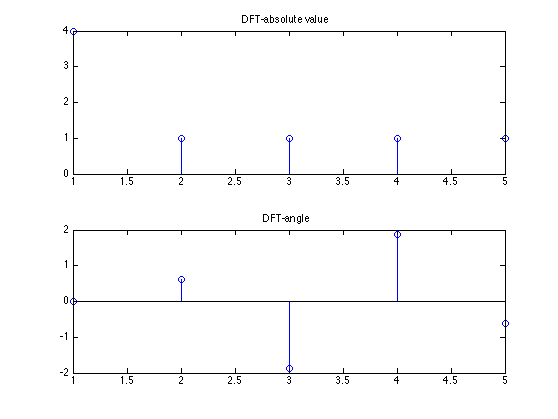
\includegraphics[scale=0.35]{dft1.png}} & 
\subfloat[DFT-B]{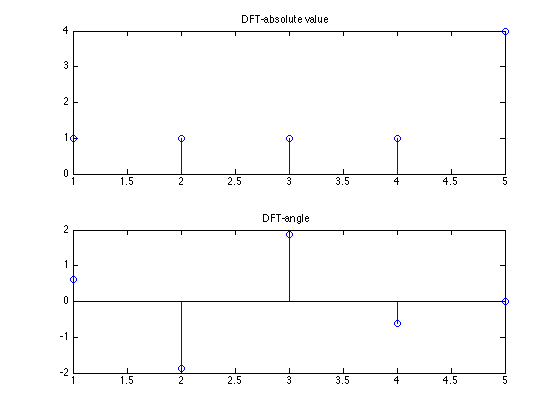
\includegraphics[scale=0.35]{dft2.png}} \\ 
\end{tabular}
\caption{Gr\'aficos de amplitud magnitud de la DFT de cada vector}
\end{figure}
\item Con base en la definici\'on de DFT muestre que la transfromada de la
se\~nal $y_n=e{{\frac{i2r\pi}{5}}n}x_n$ est\'a dada por: $Y_k=X_{k-r}$

Si se tiene un se\~nal $y_n=e{{\frac{i2r\pi}{N}}n}x_n$, por definici\'on, su DFT
est\'a dada por la expresi\'on $\mbox{\bf{DFT}\rm}[y_k]=Y_k=\sum_{n=0}^{N-1}
y_ne^{{\frac{-i2n\pi}{N}}k}$ y por la definici\'on de la se\~nal $y_n$ como
dependiente de la se\~nal $x_n$ se tiene que $\mbox{\bf{DFT}\rm}[y_k]=Y_k=\sum_{n=0}^{N-1}
[e{{\frac{i2r\pi}{N}}n}x_n]e^{{\frac{-i2n\pi}{N}}k}=\sum_{n=0}^{N-1}
=\sum_{n=0}^{N-1}e{{\frac{i2n(r-k)\pi}{N}}}x_n$. 
$\mbox{\bf{DFT}\rm}[y_k]=Y_k=\sum_{n=0}^{N-1}e{{\frac{i2n(r-k)\pi}{N}}}x_n=\sum_{n=0}^{N-1}e{{\frac{-i2n(k-r)\pi}{N}}}x_n$Si
se representa $k-r$ como l, se tiene que
$\mbox{\bf{DFT}\rm}[y_k]=Y_k=\sum_{n=0}^{N-1}e{{\frac{-i2n(l)\pi}{N}}}x_n=\mbox{\bf{DFT}\rm}[x_l]=\mbox{\bf{DFT}\rm}[x_{k-r}]=X_{k-r}$.
Para entender el punto anterior a trav\'es de \'esta demostraci\'on, se tiene
que $\boldsymbol{\vec{x_n}}=[1,1,0,1,1]$ y
$\boldsymbol{\vec{y_n}}=\boldsymbol{\vec{w_n}} \boldsymbol{\vec{x_n}}$ con
$\boldsymbol{\vec{w_m}}=[1,e^{{\frac{i2\pi}{5}}},0,e^{{\frac{i6\pi}{5}}},e^{{\frac{i8\pi}{5}}}]$,
por lo tanto, para este caso $r=1$ y $\boldsymbol{\vec{y_n}}$ es expresableen la
forma necesaria para que se cumpla la f\'ormula de la demostraci\'on y por lo
tanto, la computaci\'on adecuada mostrar\'a que la DFT del segundo vector del
punto anterior cumple con lo aqu\'i demostrado.
\item Demostrar la f\'ormula de suma geom\'etrica infinita para n\'umeros
complejo.

Es clara la siguiente afirmaci\'on $\mathbb{R} \subseteq \mathbb{C}$, y se sabe
por c\'alculo elemental que la suma geom\'etrica infinita para n\'umeros reales
se cumple, por lo que debe pensarse esta y otras propiedades como una herencia
de los n\'umeros complejos, es decir sabemos que es cierta. A continuaci\'on la
demostraci\'on formal.
$$\sum_{n=0}^{\infty}z^n=\lim_{k\to\infty} \sum_{n=1}^{k} z^n=\lim_{k\to\infty} \xi \implies \xi=\sum_{n=1}^{k} z^n$$
$$\xi=1+z+z^2+\ldots+z^k \implies z\xi=z+z^2+z^3+\ldots+z^{k+1}$$ $$\implies \xi
- z\xi=(1+z+z^2+\ldots+z^k)-(z\xi=z+z^2+z^3+\ldots+z^{k+1})=1-z^{k+1}$$
$$\implies \xi(1-z)=1-z^{k+1} \implies \xi=\frac{1-z^{k+1}}{1-z}=\sum_{n=1}^{k}
z^n$$
$$\implies \sum_{n=0}^{\infty}z^n=\lim_{k\to\infty} \sum_{n=1}^{k}
z^n=\lim_{k\to\infty} \sum_{n=1}^{k} \frac{1-z^{k+1}}{1-z}$$
Para un rango abierto entre menos uno y uno se sabe que la suma converge si $k$
tiende a infinito, por lo tanto.
$$\sum_{n=1}^{k} \frac{1-z^{k+1}}{1-z}=\frac{1}{1-z}$$
\item Si la transformada $z$ se define como
$\boldsymbol{X}(z)=\sum_{n=0}^{\infty} x[n]z^{-n}$. Encuentre la transformada
$z$ para las siguientes se\~nales: $x_n=u_n$ y $x_n=u_{1-n}$.
\\Para la primera se\~nal, se tiene la siguiente proposici\'on:
$$\forall n \in \mathbb{Z} \wedge n \gtrsim 0 \implies x[n]=u_n=1 \implies
\sum_{n=0}^{\infty} x[n]z^{-n}=\sum_{n=0}^{\infty} z^{-n}=\frac{1}{1-z^{-1}} \iff z^{-1} \neq 1$$
Para la segunda se\~nal, se sabe que si el valor de $n$ es igual a cero, el
valor de la transformada $z$ ser\'a cero, si $n$ toa otro valor discreto
distinto a cero, la suma se puede escribir como $\sum_{n=1}^{\infty}
u_{n}z^{-n}$ y la siguiente proposici\'on se preserva:
$$\forall n \in \mathbb{Z} \wedge n \gtrsim 0 \implies x[n]=u_n=1 \implies
\sum_{n=1}^{\infty} x[n]z^{-n}=\sum_{n=1}^{\infty}
z^{-n}=\frac{z^{-1}}{1-z^{-1}} \iff z^{-1} \neq 1$$
$$\sum_{n=1}^{\infty}
z^{-n} =
\left\{
	\begin{array}{ll}
		0  & \mbox{si } x \leq 0 \\
		\frac{z^{-1}}{1-z^{-1}}  & \mbox{si } \neg(x \leq 0)
	\end{array}
\right.$$
\pagebreak
\item Si la DTFT de una se\~nal se define como
$\boldsymbol{X}(w)=\sum_{n=-\infty}^{\infty} x[n]e^{-jwn}$, encontrar la DTFT de
las siguientes se\~nales $x_n=2^{-n}u_n$, $x_n=2^nu_{-n}$,$x_n=2^{-jn}$.


Para la primera se\~nal, se tiene que su DTFT es
$\boldsymbol{X}(w)=\sum_{n=-\infty}^{\infty} 2^{-n}u_ne^{-jwn}$ por definici\'on
del escal\'on unitario, se tiene que:
$$n\in (-\infty,0) \implies \boldsymbol{X}(w)=0;$$
$$n\in [0, \infty) \implies \boldsymbol{X}(w)=\sum_{n=0}^{\infty}
2^{-n}e^{-jwn}=\sum_{n=0}^{\infty}(2e^{jw})^{-n}=\frac{1}{1-(2e^{jw})^{-1}}
\iff (2e^{jw})^{-1} \neq 1$$

Para la segunda DTFT, se tiene que $u_{-n}$ es una versi\'on al rev\'es del
escal\'on unitario, por lo tanto, es cero si $n$ es mayor a cero, de lo
contrario es uno, para esta \'ultima parte se tiene que
$\boldsymbol{X}(w)=\sum_{n=-\infty}^{0}(2e^{-jw})^{n}$, realizando un cambio de
variable sobre el l\'imite inferior de la suma, se tiene que
$$\boldsymbol{X}(w)=\sum_{k=0}^{\infty}(2e^{-jw})^{-k} = \sum_{k=0}^{\infty}
2^{-k}e^{jwk} = \sum_{k=0}^{\infty} \left(\frac{e^{jw}}{2} \right)^{\!k} $$
Nuevamente. usando el resultado obtendo anteriormente, se tiene que:
$$\boldsymbol{X}(w)=\frac{1}{1-\frac{e^{jw}}{2}} \iff \frac{e^{jw}}{2} \neq 1$$
La forma general de esto ser�a:
$$\left\{
	\begin{array}{ll}
		0  & \mbox{si } x > 0 \\
		\frac{1}{1-\frac{e^{jw}}{2}}  & \mbox{si } n \leq 0
	\end{array}
\right.$$

Para la \'ultima DTFT, se tiene
$\boldsymbol{X}(w)=\sum_{n=-\infty}^{\infty}
2^{-jn}e^{-jwn}=\sum_{n=-\infty}^{\infty}
(2^{-j}e^{-jw})^n=\sum_{n=-\infty}^{0}
(2^{-j}e^{-jw})^n+\sum_{n=1}^{\infty} (2^{-j}e^{-jw})^n$, sea
$\xi=2^{-j}e^{-jw}$, entonces,$\boldsymbol{X}(w)=\sum_{n=-\infty}^{0}
(\xi)^n+\sum_{n=1}^{\infty} (\xi)^n$
Por manipulaciones con las propiedades de la sumatoria y algunos cambios de
variable, se llega a:
$$\boldsymbol{X}(w)=\sum_{n=-\infty}^{0}
(\xi)^n+\sum_{n=1}^{\infty} (\xi)^n=\sum_{k=0}^{\infty}
(\xi)^{-k}+\frac{\xi}{1-\xi}$$
$$=\sum_{k=0}^{\infty}
(2^{-j}e^{-jw})^{-k}+\frac{2^{-j}e^{-jw}}{1-2^{-j}e^{-jw}}=\sum_{k=0}^{\infty}2^{-jk}e^{-jwk}+\frac{2^{-j}e^{-jw}}{1-2^{-j}e^{-jw}}$$
$$=\sum_{k=0}^{\infty}[\frac{1}{2^{j}e^{jw}}]^k+\frac{2^{-j}e^{-jw}}{1-2^{-j}e^{-jw}}=
\sum_{k=0}^{\infty}[\frac{1}{(2e^w)^j}]^k+\frac{2^{-j}e^{-jw}}{1-2^{-j}e^{-jw}}$$
$$=\frac{1}{1-\frac{1}{(2e^w)^j}}+\frac{2^{-j}e^{-jw}}{1-2^{-j}e^{-jw}}=\frac{1}{1-\frac{1}{(2e^w)^j}}
+\frac{1}{(2e^w)^j(1-\frac{1}{(2e^w)^j})} \iff (2e^w)^j) \neq 1$$
\pagebreak
\\
A continuaci\'on, se muestran las gr\'aficas de las primeras dos transformadas.
\begin{figure}
\centering
\begin{tabular}{cc}
\subfloat[DFT-A]{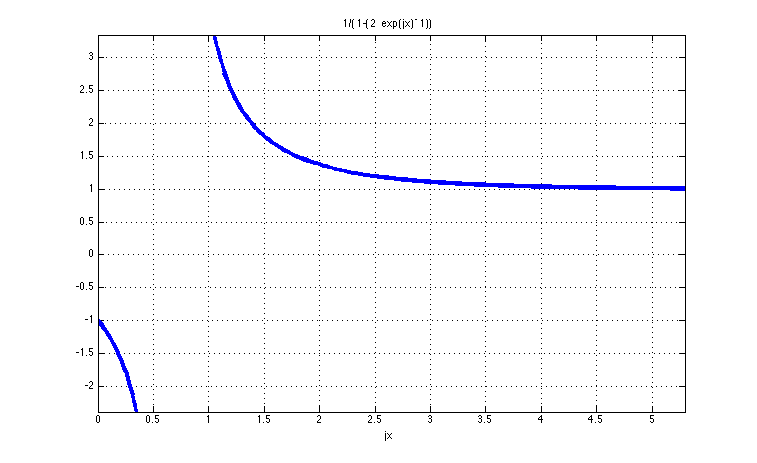
\includegraphics[scale=0.25]{d1.png}} & 
\subfloat[DFT-B]{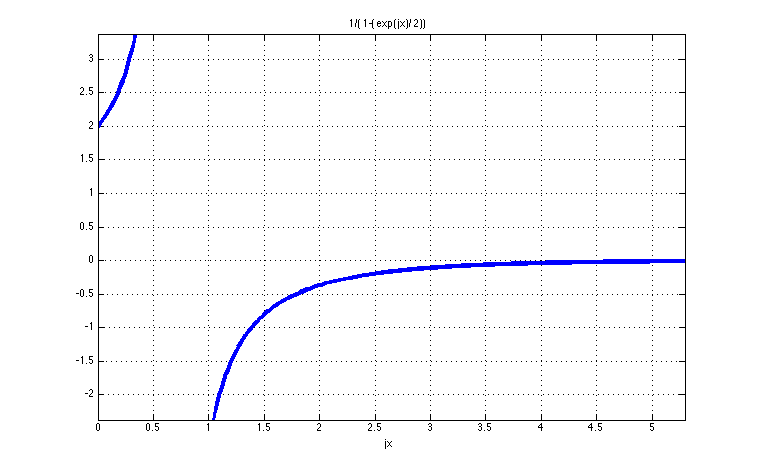
\includegraphics[scale=0.25]{d2.png}} \\ 
\end{tabular}
\caption{Gr\'aficos las DTFT de cada vector}
\end{figure}

\item Encuentre y grafique la DTFT de las se\~nales $\delta_n$, $u_{n-1}-u_{+1}$
y $\delta_n-\delta_{n-1} $\\
Como $\delta_n$, tiene un valor distinto a cero s\'i y s\'olo si n es cero, el
valor de la DTFT es la unidad. La segunda se\~nal, consiste en un pulso negativo
entre menos uno y uno, por lo tanto, para $n$ fuera de esta rango cualqquier
producto por esta se\~nal es cero, por lo tanto, la DTFT se reduce a
$\boldsymbol{X}(e^{jw})=\sum_{n=-1}^{1} e^{-jwn}=e^{jw}+1+e^{-jw}$. Finalmente,
la \'ultima se\~nal es un pulso en cero y uno negativo en uno; por linealidad de
la DTFT, su transformada ser\'a $1+e^{jw}$. A continuaci\'on se ilustran las
gr\'aficas.
\begin{figure}
\centering
\begin{tabular}{cc}
\subfloat[DTFT-A]{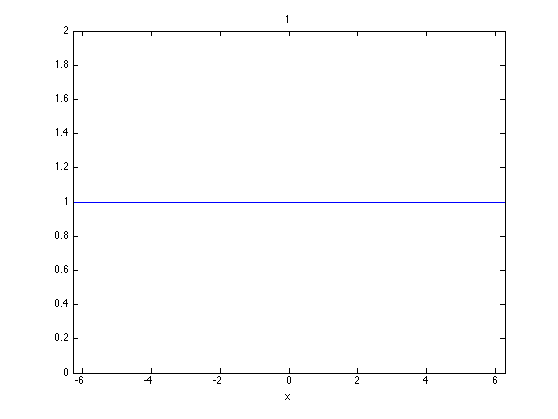
\includegraphics[scale=0.25]{t1.png}} & 
\subfloat[DTFT-B]{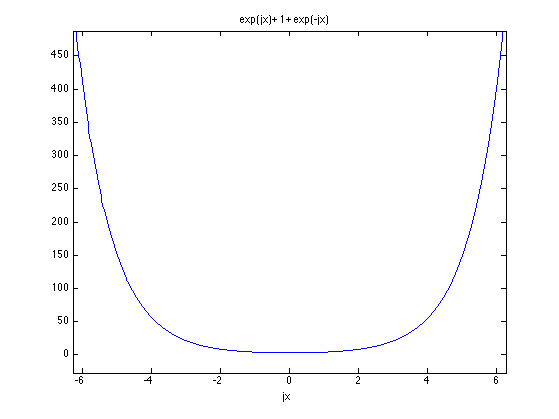
\includegraphics[scale=0.25]{t2.png}} &
\subfloat[DTFT-C]{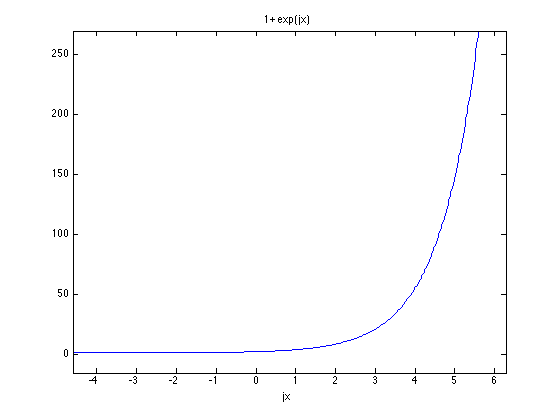
\includegraphics[scale=0.25]{t3.png}} \\
\end{tabular}
\caption{Gr\'aficos las DTFT de cada vector}
\end{figure}
\pagebreak
\item Qu\'e relaci\'on existe entre la DFTF y la transformada $z$
\\La transformada $z$, definida como $\boldsymbol{X}(z)=\sum_{n=\infty}^{\infty}
x[n]z^{-n}$ y la DTFT se define como
$\boldsymbol{X}(e^{jw})=\sum_{n=-\infty}^{\infty} x[n]e^{-jwn}$, sea
$z=re^{jw}$, si se remplaza esto en la expresi\'on de la transformada $z$, se
tiene $$\boldsymbol{X}(z)=\sum_{n=\infty}^{\infty}
x[n](re^{jw})^{-n}=\boldsymbol{X}(z)=\sum_{n=\infty}^{\infty}
(x[n]r^{-n})e^{-jwn}$$ Lo cual revela que la transformada $z$ es la DTFT de
$x[n]r^{-n}$










\end{enumerate}
\end{document}